\section{Ergebnisse}


\subsection{Ergebnisse der statischen Tests}
\begin{flushleft}
Im Folgenden werden die Ergebnisse der statischen Tests mit Bezug auf Temperatur- und Leistungsverlauf mehrerer Wandler dargestellt und näher erläutert. Der Versuchsaufbau und die Testumgebung waren bei allen drei Wandlern nahezu identisch. 
In Abb. 10 ist der Temperaturverlauf [in °C] von drei unterschiedlichen Wandlern  über einen Zeitverlauf von 3600 Sekunden aufgetragen. Es ist zu erkennen, dass der Wandler mit der Bezeichnung 'Board\_10' eine wesentlich höhere Einschwingtemperatur besitzt als die anderen zwei. Dies lässt sich darauf zurückführen, dass besagter Wandler \hl{einen Hardware defekt besitzt}. Des Weiteren ist zu erkennen, dass die beiden verbleibenden Wandler trotz identischer Hardware und gleichen Testbedingungen unterschiedliche Temperaturen vorweisen. \hl{Somit kann behauptet werden, das unter gleichen Bedingungen Abweichende Resultate herauskommen können.}
\end{flushleft}

\begin{figure}[H]
    \centering
    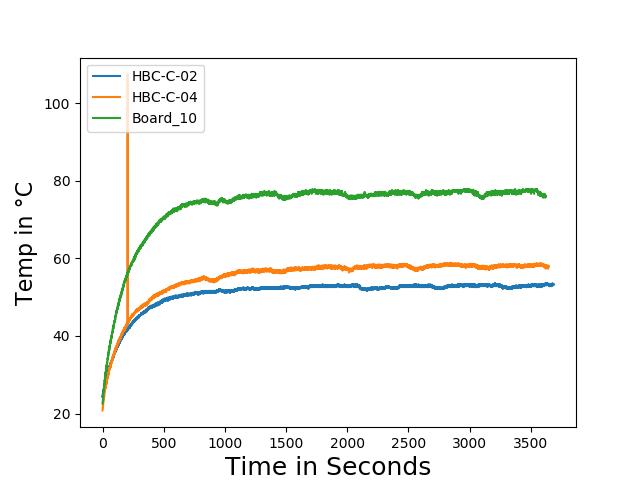
\includegraphics[height= 6cm, width = 12cm]{Pictures/3_Boards_Temp.png}
    \caption{Temperaturvergleich mehrerer Wandler}
\end{figure}


\begin{flushleft}

In \hl{Abb. x} ist der Leistungsverlauf [in Watt] der drei Wandler geplotet gegen die [Zeit in Sekunden] zu sehen. Aus diesem Graphen ist sofort ersichtlich, dass alle Signale rauschen. Wie man \hl{Tabelle X} entnehmen kann, beträgt die Standardabweichung vom Mittelwert bei allen Signalen \hl{Ungefähr 300 Milliwatt}. Die theoretische Leistung, welche bei einer Spannung von 12 V und zwei Parallel geschalteten Widerständen (siehe 3.1) generiert werden müsste, beträgt 61.2 Watt: 

\begin{equation}[H]
\label{Ohmsches Gesetz}
12 V * 5.1 A = 61.2 W 
\end{equation} 

Somit liegt der Wandler mit der Bezeichnung "HB-C-02" am nächsten zum theoretisch berechneten Wert. Diese praktische Abweichung kann durch \hl{einen Leistungsabfall in den Leitungskabeln und der Hardware zumindest teilweise erklärt werden.}

Aufgrund dieser Resultate ist es für Maschine Learning Applikationen sinnvoll auf diese Daten einen Frequenzfilter anzuwenden, um das Rauschen zu eliminieren, da ansonsten Inkonsistenzen bei den K.I Applikationen vorkommen können, da die Daten unter gleichen Bedingungen variieren. 

\end{flushleft}

\begin{figure}[H]
    \centering
    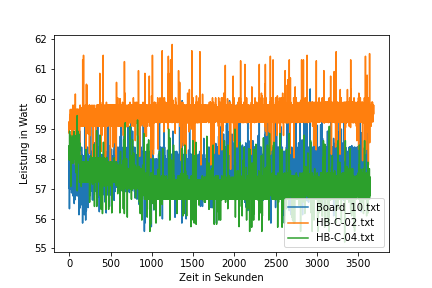
\includegraphics[height= 6cm, width = 12cm]{Pictures/3_Boards_Leistung.png}
    \caption{Leistungsvergleich mehrerer Wandler}
\end{figure}



In \hl{Abb. x} ist der Leistungsverlauf zu erkennen, auf den ein Tiefpassfilter angewendet wurde. Bei dem Tiefpassfilter handelt es sich um \hl{Blablabla details}. Dieser Datensatz besitzt nun kein Rauschen mehr, die einzelnen Signale sind jedoch trotzdem noch unterscheidbar. 


\begin{figure}[H]
    \centering
    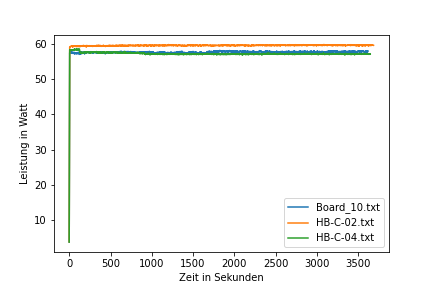
\includegraphics[height= 6cm, width = 12cm]{Pictures/3_Board_Leistung_Filtered.png}
    \caption{Gefilterter Leistungsverlauf der drei Wandler}
\end{figure}

\begin{flushleft}



\subsection{Ergebnisse der dynamischen Tests}
Zur dynamischen Datenerfassung ist zu sagen, dass das I²C Protokoll sich limitierend darauf ausgewirkt hat. Dadurch, dass stabile Programmausführung nur bei einer I²C Taktrate von 70 KHz gewährleistet war, war die Konsequenz daraus, dass die Abtastrate ebenfalls reduziert wurde. Die Ermittlung der Abtastrate erfolgte durch Messungen mehrerer Wandler, die mit verschiedenen Signalen gespeist wurden.Wie in Abb. 13 zu erkennen ist, wurden zwei verschiedene Wandler mit jeweils 6 verschiedenen Signalen verwendet. Zur Bestimmung der jeweiligen Abtastrate wurde zu durch Zeitstempel das Zeitdelta bestimmt, d. h. der Zeitraum in dem die Messungen durchgeführt wurden. Anschließend wurde die Anzahl der aufgenommenen Samples durch das Zeitdelta geteilt, um so auf die durchschnittliche Abtastrate zu kommen. Darauffolgend wurde der Mittelwert von allen Wandler-Signal Paaren berechnet, welcher ~110 Hz beträgt. Wenn auf dieses Ergebnis die oben genannten Konzepte der Nyquist Frequenz angewendet werden, so zeigt sich, dass die maximale Signalfrequenz, welche ohne Verzerrungen durch den Wandler abgetastet werden kann, bei 55 Hz liegt. Aus diesem Grund wurden im nachfolgenden Test mit einem Neuronalen Netz nur Signalfrequenzen verwendet, welche einen geringere Frequenz als 55 Hz besitzen. 

\begin{figure}[H]
    \centering
 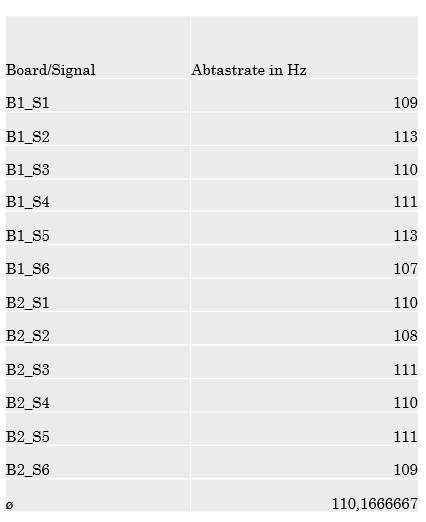
\includegraphics[height= 6cm, width =4 cm]{Pictures/Speed.png}
    \caption{Berechnung der Abtastrate}
\end{figure}


In Abb. 4 ist das generierte Signal zu sehen, welches in den Verstärker eingespeist wird. Dabei handelt es sich in diesem Beispiel um ein 10 Hz Sinussignal, welches in Audacity generiert wurde und als Signalinput für den Stereo-Verstärker dient. Dadurch, dass der Verstärker sowohl positive als auch negative Signale verstärkt, ergibt sich für die reine Leistungsaufnahme des Wandlers eine theoretische Leistungskurve wie sie in Abb. 11 dargestellt ist, nämlich  der Betrag einer Sinusfunktion:

\begin{equation}[H]
f(x) = |sin(2 * pi*x*10)|
\end{equation}

Dadurch, dass es vorher ein Sinussignal mit einer Frequenz von 10 Hz war, ist es nun ein Sinussignal mit einer effektiven Frequenz von 20 Hz.

Das Messen der Daten erfolgte auf einem Raspberry Pi per I²C Protokoll und einer eingestellten Taktrate von 70 KHz, da diese Stabilität gewährleistet. Die Datenerhebung und Verarbeitung erfolgte durch die Programmiersprache Python.

\begin{figure}[H]
    \centering
    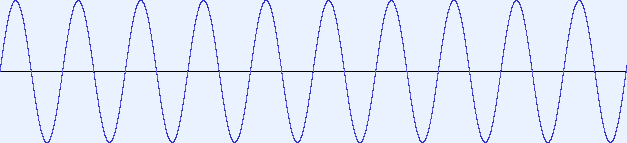
\includegraphics[height= 4cm, width = 12cm]{Pictures/Sinus_Aud.png}
    \caption{In Audacity generiertes 10 Hz Sinussignal}
\end{figure}

\begin{figure}[H]
    \centering
    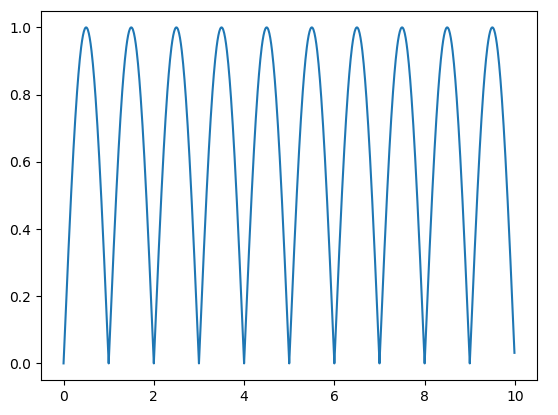
\includegraphics[height= 4cm, width = 12cm]{Pictures/Clapped_Sine.png}
    \caption{Effektive Frequenz eines 10 Hz Signals ist 20 Hz, weil, weil es für den Verstärker egal ist ob + oder - Signal }
\end{figure}

\begin{figure}[H]
    \centering
    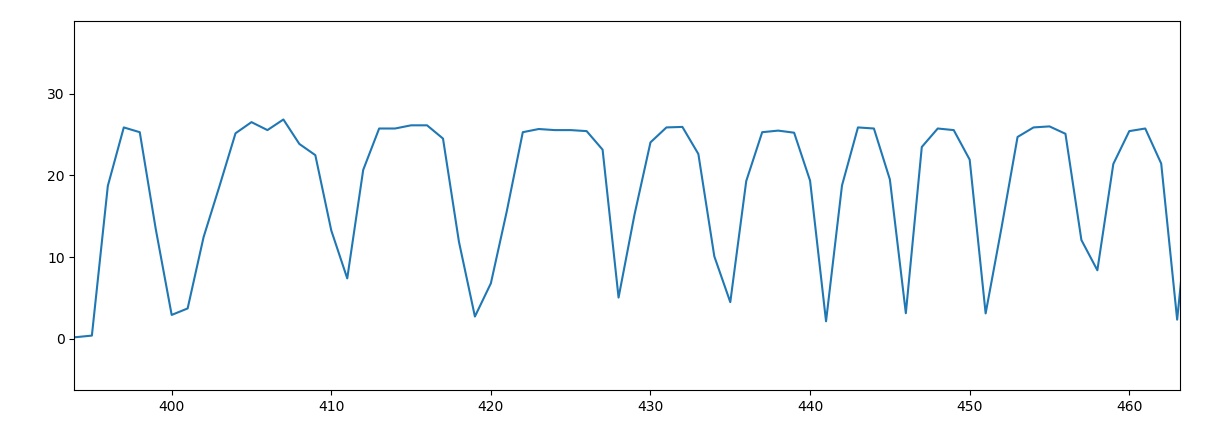
\includegraphics[height= 4cm, width = 12cm]{Pictures/TatsDaten.png}
    \caption{Tatsächlich gemessene Leistung des Wandlers}
\end{figure}


In Abb. 6 ist der ungefilterte Leistungsverlauf des Wandler dargestellt. Es ist ersichtlich, dass das umgeklappte 20 Hz Sinussignal in Abb. 5, dem gemessenen Sinussignal, entspricht. Der unsaubere Verlauf der Leistung ist auf Rauschen innerhalb der Hardware und auf die geringe Abtastrate von 110 Hz zurückzuführen. 


\subsection{Ergebnis des Anwendbarkeitstest - Neuronales Netz}

Als Architektur des Neuronalen Netzes wurde ein Netz mit einem Input layer, zwei Hidden layern, sowie einem Output layer gewählt. Als Aktivierungsfunktion der Neuronen wurde ReLu ausgewählt, die Output Neuronen werden durch die softmax Funktion Aktiviert. Der verwendete Optimierungsalgorithmus ist Gradient Descent. Als Input Daten wurden 50 Samples des zeitlichen Leistungsverlaufs eines Signals verwendet. Die Ausgabe des Neuronalen Netzes ist eine Klassifizierung, um was für eine Signalfrequenz es sich bei den Input Daten handelt. 


Abb. 13 zeigt die Genauigkeit des Neuronalen Netzes in der Vorhersage der verschiedenen Frequenzen anhand der Trainingsdaten. Es ist aus dem Graphen ersichtlich, dass die Genauigkeit über 1000 Trainingsepochen ~99\% beträgt. 


\begin{figure}[H]
    \centering
    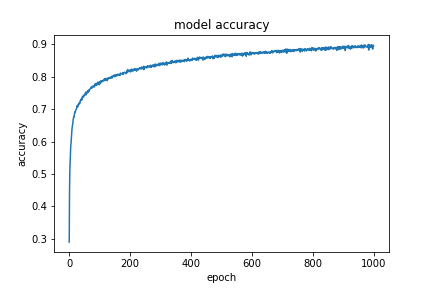
\includegraphics[height= 4cm, width = 8cm]{Pictures/Loss.png}
    \caption{Genauigkeit der Anwendbarkeitstests}
\end{figure}
